\subsection{LZ78}

\begin{frame}{\FrameName}
\begin{block}{LZ78 - Datenstrukturen}
	\begin{itemize}[<+->]
		\item Strings werden als Sequenzen von Paaren $(i,c)$ dargestellt \linebreak \Hint{$i$...Index eines Vorgänger-Paares oder $0$$; c \in \Sigma$}
		\item Jedes Paar repräsentiert einen Substring
		\item Wenn $i$ gleich $0$ dann ist dieser Substring gleich $c$
		\item Andernfalls ist der Substring des $i$-ten Parres gefolgt von $c$
	\end{itemize}
\end{block}
\end{frame}

\begin{frame}{\FrameName}
\begin{block}{Beispiel}
	\Gap
	\Gap
	\only<1>{
		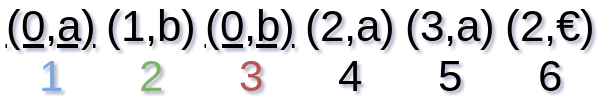
\includegraphics[width=\textwidth]{Images/LZ78/blank}}
	\only<2>{
		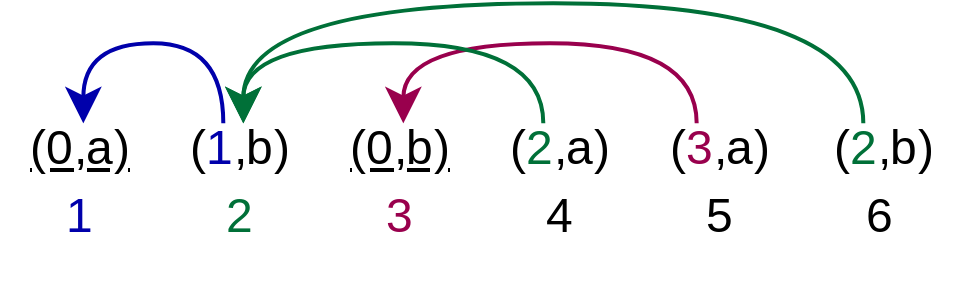
\includegraphics[width=\textwidth]{Images/LZ78/withRef}}
	\only<3>{
		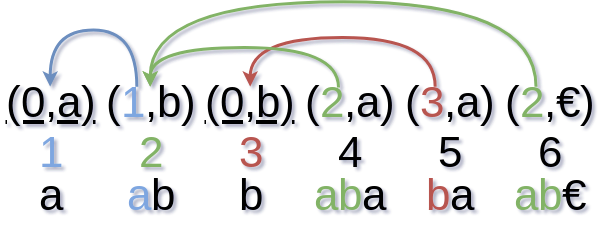
\includegraphics[width=\textwidth]{Images/LZ78/full}}
\end{block}
\end{frame}

\begin{frame}{\FrameName}
\begin{block}{LZ78 - Algorithmus}
	\begin{itemize}[<+->]
		\item String wird Schrittweise in einem Durchlauf von links nach rechts in eine Sequenz von Paaren übersetzt
		\item Finde in jedem Schritt das kürzeste Präfix $\gamma$ des verbleibenden Strings das nicht Expansion eines bereits erzeugten Paars ist
		\item Am Ende des Strings muss eventuell ein weiteres Zeichen hinzugefügt werden
		\item Ein neues Paar wird an die Liste angehangen:
		\begin{enumerate}
			\item<4-> Wenn da $\gamma = 1$ ist füge $(0,\gamma)$ hinzu
			\item<5-> Andernfalls ist $\gamma = \alpha c$. \linebreak $\alpha$ ... Expansion eines Paars mit dem Index $i_\alpha$ \linebreak $\Rightarrow$ Paar: $(i,c)$
		\end{enumerate}
	\end{itemize}
\end{block}
\end{frame}

% Marking string sequence
\newcommand{\M}[1]{\textcolor{OrangeRed}{#1}}

\begin{frame}{\FrameName}
\begin{block}{Beispiel}
	\begin{description}[<+->]
		\item \M{a}abbababaab\euro
		\item (0,a) \M{ab}bababaab\euro
		\item (0,a) (1,b) \M{b}ababaab\euro
		\item (0,a) (1,b) (0,b) \M{aba}baab\euro
		\item (0,a) (1,b) (0,b) (2,a) \M{ba}ab\euro
		\item (0,a) (1,b) (0,b) (2,a) (3,a) \M{ab\euro}
		\item (0,a) (1,b) (0,b) (2,a) (3,a) (2,\euro)
	\end{description}
\end{block}
\end{frame}

\begin{frame}{\FrameName}
\begin{block}{LowerBound}
	\begin{center}
		\fbox{$ \alpha_k = a^{k(k+1)/2}(ba^k)^{(k+1)^2} $}
	\end{center}
	\begin{itemize}[<+->]
		\item $|\alpha_k | = k \frac{k+1}{2} + (1+k)(k+1)^2$ \linebreak
			$\phantom{|\alpha_k |} = k^3 + \frac{7}{2}k^2 + \frac{7}{2}k + 1$
		\item $ n = |\alpha_k | \in \Theta(k^3)$
	\end{itemize}
\end{block}
\end{frame}

\begin{frame}{\FrameName}
\begin{block}{UpperBound $m^*$}
	\begin{center}
		\fbox{$ \alpha_k = a^{k(k+1)/2}(ba^k)^{(k+1)^2} $}
	\end{center}
	\begin{itemize}[<+->]
		\item $m^* \in \mathcal{O}(1+ log(\frac{k^2+k}{2}) + log(k+1)^2 + 1+ log(k))$
		\item $m^* \in \mathcal{O}(log \thinspace k)$
		\item $m^* \in \mathcal{O}(log \thinspace n^\frac{1}{3}) = \mathcal{O}(log \thinspace n)$
	\end{itemize}
\end{block}
\end{frame}

\begin{frame}{\FrameName}
\begin{block}{LowerBound m}
	\begin{center}
		\fbox{$ \alpha_k = a^{k(k+1)/2}(ba^k)^{(k+1)^2} $}
	\end{center}
	\begin{itemize}[<+->]
		\item String wird in zwei Phasen in eine Paar-Sequenz übersetzt
		\item Erste Phase: alle Strings $a...a^k$ zu Paaren übersetzt
		\item Zweite Phase: $a^iba^j$ für alle $i,j \in [0,k]$ wird ein Paar erstellt
		\item $m \in \Omega(\sum_{z=1}^k z + (k+1)^2) = \Omega(k^2)$
		\item $m \in \Omega(n^{2/3})$
	\end{itemize}
\end{block}
\end{frame}

\begin{frame}{\FrameName}
\begin{block}{LowerBound}
	\begin{center}
		\fbox{$ \alpha_k = a^{k(k+1)/2}(ba^k)^{(k+1)^2} $}
	\end{center}
	\begin{itemize}[<+->]
		\item $m^* \in \mathcal{O}(log \thinspace n)$
		\item $m \in \Omega(n^{2/3})$
		\item $a(n) \in \Omega(\frac{n^{2/3}}{log \thinspace n})$
	\end{itemize}
\end{block}
\end{frame}